\documentclass[13pt,a4paper]{extarticle}
\usepackage[utf8]{inputenc}
\usepackage[utf8]{vietnam} %Bien dich duoc tieng Viet
\usepackage{amsmath,amsfonts,amssymb} %Font toan
\usepackage{type1cm}
\usepackage{times}
\usepackage{graphicx}
\graphicspath{ {images03/} }
\usepackage{enumerate}
\usepackage{comment}
\usepackage{multicol}
\usepackage{multirow}
%\usepackage[unicode]{hyperref} %Tu dong tao bookmark
\usepackage[unicode, hidelinks=true]{hyperref}
\usepackage{indentfirst} %Thut vao dau dong o tat ca cac doan
\usepackage{listings} %Dinh dang code
\usepackage{color} %Mau sac
\usepackage[left=2.5cm,right=2.5cm,top=2.5cm,bottom=2.5cm]{geometry} %Canh lề trái - phải - trên - dưới cho tài liệu
\usepackage{longtable}
\renewcommand{\arraystretch}{1.3}

\begin{document}
\pagenumbering{gobble}
\title{\Large{\textbf{BÀI CHUẨN BỊ THỰC TẬP ĐIỆN CÔNG NGHIỆP}}\\\vspace{1cm}\textbf{Bài 3}\\\vspace{.5cm}\textbf{VẬN HÀNH ĐỘNG CƠ KHÔNG ĐỒNG BỘ MỘT PHA}}
\date{Ngày 26 tháng 05 năm 2016}
%\date{\today}
\author{GVHD: Võ Minh Thiện \vspace{.6cm}\\  Nhóm SVTH: Nhóm 2 -- Tiểu nhóm 1: Thi Minh Nhựt}
\maketitle
\tableofcontents
\newpage
\pagenumbering{arabic}
\setcounter{page}{1}
\section{Chuẩn bị}
VOM kim, VOM kìm và mô hình vận hành động cơ.
\section{Vận hành động cơ không đồng bộ một pha}
\subsection{Vận hành động cơ không đồng bộ một pha với tụ khởi động}\label{Sec:1tu}
Thực hiện theo các bước sau:
\begin{list}{--}{}
\item \textit{Bước 1}: Xác định cực tính và đấu dây động cơ theo hình ~\ref{khoi-dong-2tu}. Sử dụng tụ dầu.
\begin{figure}[!h]
\begin{center}
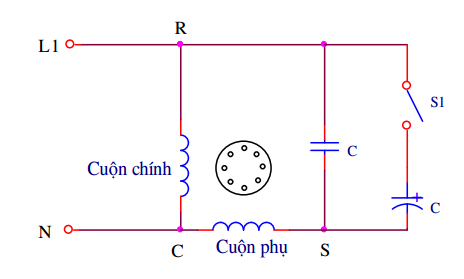
\includegraphics[scale=.5]{khoi-dong-2tu}
\end{center}
\caption{Đấu dây động cơ với tụ khởi động}\label{khoi-dong-tu}
\end{figure}
\begin{list}{+}{}
\item Xác định cực tính: do động cơ đước quấn cho 2 kiểu mắc tụ (tụ đề và tụ ngậm) nên đo điện trở thì cuộn dây phụ sẽ có điện trở lớn hơn điện trở của cuộn dây chính.
\item Khi đo đầu dây công tắc ly tâm thì điện trở của nó là 0.
\end{list}
\item \textit{Bước 2}: Lắp mạch động lực và mạch điều khiển theo sơ đồ hình ~\ref{mach-dong-luc-tu-de}.
\begin{figure}[!h]
\begin{center}
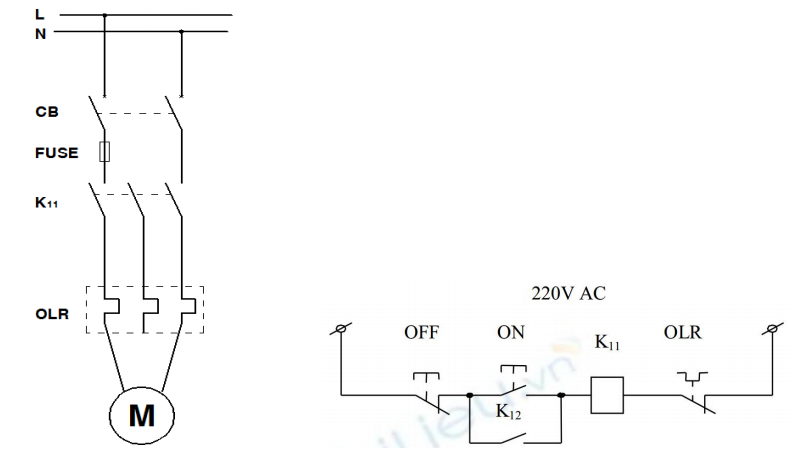
\includegraphics[scale=.6]{mach-dluc-dkhien}
\end{center}
\caption{Mạch động lực và mạch điều khiển}\label{mach-dong-luc-tu-de}
\end{figure}
\item \textit{Bước 3}: Nhờ GVHD kiểm tra, bật CB và nhấn nút ON để vận hành mô hình.
\item \textit{Bước 4}: Ghi nhận lại hiện tượng và lấy các số liệu sau điền vào bảng.
\begin{center}
\begin{tabular}{|c|c|c|c|}\hline
\textit{Điện áp vận hành} & \textit{Dòng khởi động} & \textit{Dòng không tải} & \textit{Công suất không tải}\\ 
$V$ & $A$ & $A$ & $W$ \\ \hline
& & & \\ \hline
& & & \\ \hline
\end{tabular}
\end{center}
\item \textit{Bước 5}: Nhấn nút $OFF$ để kết thúc vận hành và tắt nguồn CB.
\end{list}
\newpage
\subsection{Động cơ không đồng bộ một pha kết hợp tụ ngậm và tụ đề}
Thực hiện theo các bước:
\begin{list}{--}{}
\item \textit{Bước 1}: Từ cách đấu cực tính đã đấu cho động cơ ở mục ~\ref{Sec:1tu}, tiến hành đấu thêm tụ ngậm theo sơ đồ hình \ref{khoi-dong-2tu}.
\begin{figure}[!h]
\begin{center}
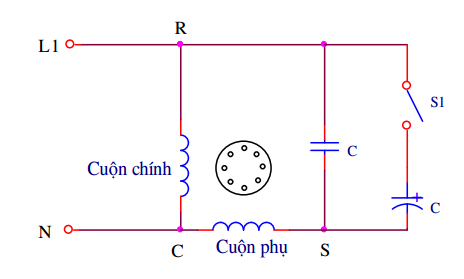
\includegraphics[scale=.4]{khoi-dong-2tu}
\end{center}
\caption{Đấu dây động cơ khởi động với 2 tụ}\label{khoi-dong-2tu}
\end{figure}
\item \textit{Bước 2}: Lắp mạch động lực và mạch điều khiển theo sơ đồ hình ~\ref{mach-dong-luc-2tu}.
\begin{figure}[!h]
\begin{center}
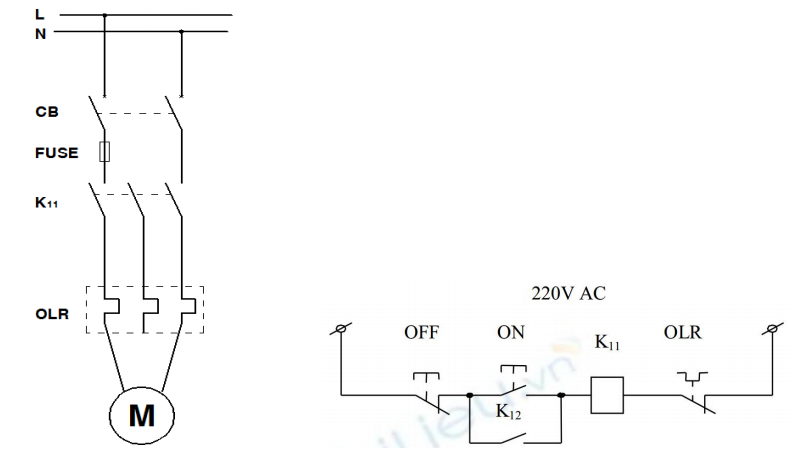
\includegraphics[scale=.6]{mach-dluc-dkhien}
\end{center}
\caption{Mạch động lực và mạch điều khiển}\label{mach-dong-luc-2tu}
\end{figure}
\item \textit{Bước 3}: Nhờ GVHD kiểm tra, bật CB và nhấn nút ON để vận hành mô hình.
\item \textit{Bước 4}: Ghi nhận lại hiện tượng và lấy các số liệu sau điền vào bảng.
\begin{center}
\begin{tabular}{|c|c|c|c|}\hline
\textit{Điện áp vận hành} & \textit{Dòng khởi động} & \textit{Dòng không tải} & \textit{Công suất không tải}\\ 
$V$ & $A$ & $A$ & $W$ \\ \hline
& & & \\ \hline
& & & \\ \hline
\end{tabular}
\end{center}
\item \textit{Bước 5}: Nhấn nút $OFF$ để kết thúc vận hành và tắt nguồn CB.
\end{list}
\section{Động cơ không đồng bộ ba pha vận hành ở lưới điện một pha}
\begin{list}{--}{}
\item \textit{Bước 1}: Xác định cực tính của các cuộn dây của động cơ 3 pha.
\begin{list}{+}{}
\item Dùng VOM (thang $\times 1 \Omega$) xác định 2 đầu dây của một cuộn dây. Gọi các cuộn lần lượt là $AX, BY, CZ$.

Ở bước này, ta chưa xác định được đầu cuối của cuộn dây
\item Đánh dấu số thứ tự cho 2 đầu dây của các cuộn: $AX \longleftrightarrow 12$, $BY \longleftrightarrow 34$ và $CZ \longleftrightarrow 56$.
\item Mắc 2 đầu của một cuộn dây vào 2 đầu của pin 9V thông qua \textit{công tắc}, chuyển VOM sang thang đo $mA$:
\begin{list}{$\ast$}{}
\item Giả sử: $AX = 12$, cần xác đinh cặp $34 = ??$
\item Đặt que đen: số 3; que đỏ: số 4. Đóng công tắc.
\item Nếu kim quay theo chiều thuận và về 0 thì: $34=BY$, ngược lại thì $34 = YB$.
\item Xác định cặp $56 = ??$, thực hiện tương tự.
\item[$\Longrightarrow$] Vì quá trình đóng công tắc thì dòng điện mới biến thiên (xảy ra quá trình quá độ trong mạch).
\end{list}
\end{list}
\item \textit{Bước 2}: Đâu dây động cơ như sơ đồ hình \ref{3p-1p}.
\begin{figure}[!h]
\begin{center}
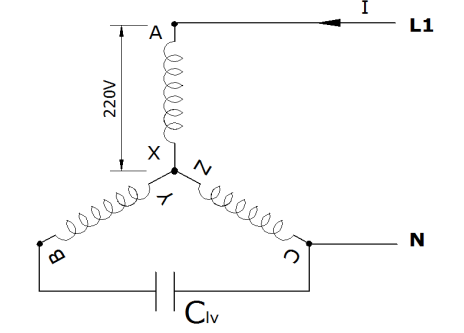
\includegraphics[scale=.6]{3p-1p-Y}
\end{center}
\caption{Đấu dây động 3 pha cơ chạy chế độ 1 pha}\label{3p-1p}
\end{figure}
\item \textit{Bước 3}: Lắp mạch động lực và mạch điều khiển theo sơ đồ hình ~\ref{mach-dong-luc-tu-de}.
\begin{figure}[!h]
\begin{center}
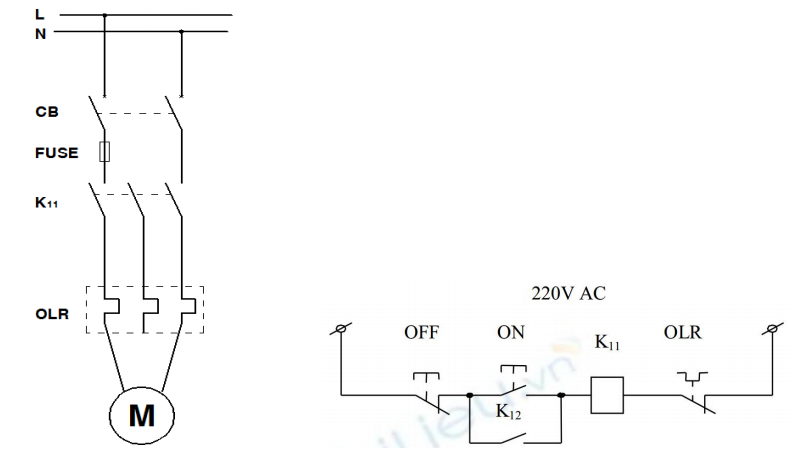
\includegraphics[scale=.6]{mach-dluc-dkhien}
\end{center}
\caption{Mạch động lực và mạch điều khiển}\label{mach-dong-luc-tu-de}
\end{figure}
\item \textit{Bước 4}: Nhờ GVHD kiểm tra, bật CB và nhấn nút ON để vận hành mô hình.
\item \textit{Bước 5}: Ghi nhận lại hiện tượng và lấy các số liệu sau điền vào bảng.
\begin{center}
\begin{tabular}{|c|c|c|c|}\hline
\textit{Điện áp vận hành} & \textit{Dòng khởi động} & \textit{Dòng không tải} & \textit{Công suất không tải}\\ 
$V$ & $A$ & $A$ & $W$ \\ \hline
& & & \\ \hline
& & & \\ \hline
\end{tabular}
\end{center}
\item \textit{Bước 6}: Nhấn nút $OFF$ để kết thúc vận hành và tắt nguồn CB.
\end{list}
\newpage
\section{Động cơ 1 pha khởi động bằng điện trở phụ}
\begin{list}{--}{}
\item \textit{Bước 1}: Chuẩn bị động cơ 2 pha $220V/380V$, $2.2kW$ có tích hợp sẳn điện trở máy.
\item \textit{Bước 2}: Xác định cực tính của động cơ và đấu sơ đồ như hình ~\ref{R-phu-thuan}.
\begin{figure}[!h]
\begin{center}
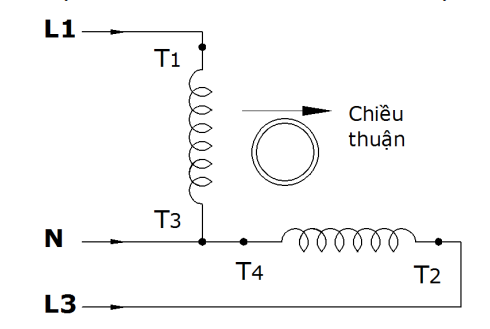
\includegraphics[scale=.6]{R-phu-thuan}
\end{center}
\caption{Sơ đồ đấu dây động cơ vận hành chiều thuận}\label{R-phu-thuan}
\end{figure}
\item \textit{Bước 3}: Lắp mạch động lực và mạch điều khiển theo sơ đồ hình ~\ref{mach-dong-luc-tu-de}.
\begin{figure}[!h]
\begin{center}
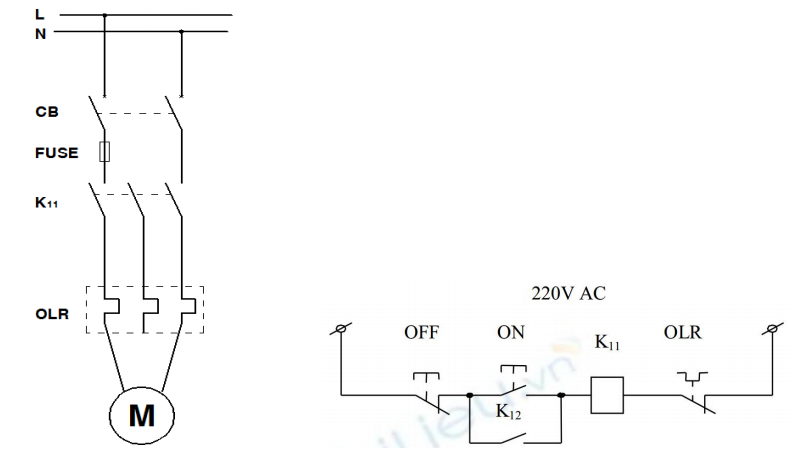
\includegraphics[scale=.6]{mach-dluc-dkhien}
\end{center}
\caption{Mạch động lực và mạch điều khiển}\label{mach-dong-luc-tu-de}
\end{figure}
\item \textit{Bước 4}: Nhờ GVHD kiểm tra, bật CB và nhấn nút ON để vận hành mô hình.
\item \textit{Bước 5}: Ghi nhận lại hiện tượng và lấy các số liệu sau điền vào bảng.
\begin{center}
\begin{tabular}{|c|c|c|c|}\hline
\textit{Điện áp vận hành} & \textit{Dòng khởi động} & \textit{Dòng không tải} & \textit{Công suất không tải}\\ 
$V$ & $A$ & $A$ & $W$ \\ \hline
& & & \\ \hline
& & & \\ \hline
\end{tabular}
\end{center}
\item \textit{Bước 6}: Nhấn nút $OFF$ để kết thúc vận hành và tắt nguồn CB.
\item \textit{Bước 7}: Vận hành đảo chiều bầng cách chuyển pha động cơ theo hình ~\ref{R-phu-nghich}.
\begin{figure}[!h]
\begin{center}
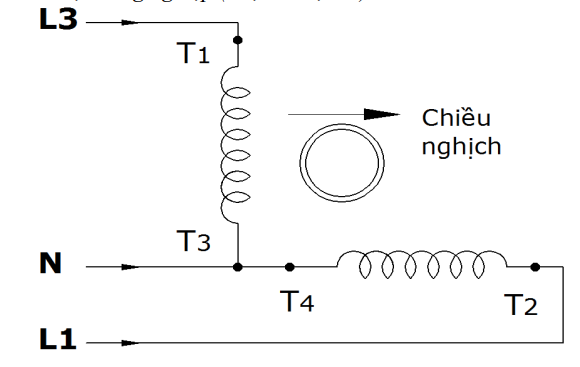
\includegraphics[scale=.5]{R-phu-nghich}
\end{center}
\caption{Sơ đồ đấu dây động cơ vận hành chiều nghich}\label{R-phu-nghich}
\end{figure}

Ở sơ đồ \textit{hình \ref{R-phu-thuan}} cấp nguồn $L1-L3$; ở sơ đồ \textit{hình \ref{R-phu-nghich}} cấp nguồn $L3-L1$, nên động cơ sẽ đảo chiều quay.
\item \textit{Bước 8}: Nhờ GVHD kiểm tra, bật CB và nhấn nút ON để vận hành mô hình.
\item \textit{Bước 9}: Ghi nhận lại hiện tượng và lấy các số liệu sau điền vào bảng.
\begin{center}
\begin{tabular}{|c|c|c|c|}\hline
\textit{Điện áp vận hành} & \textit{Dòng khởi động} & \textit{Dòng không tải} & \textit{Công suất không tải}\\ 
$V$ & $A$ & $A$ & $W$ \\ \hline
& & & \\ \hline
& & & \\ \hline
\end{tabular}
\end{center}
\item \textit{Bước 10}: Nhấn nút $OFF$ để kết thúc vận hành và tắt nguồn CB.
\end{list}
\end{document}